\section{Auswertung}
\label{sec:Auswertung}
Zur Bestimmung des Lande-Faktors der Elektronen und des Erdmagnetfeldes in Dortmund, werden zunächst die x-Koordinaten in Abbildung \ref{fig:Skizze} zu sehenden Graphen normiert.
\begin{figure}
  \centering
  \begin{subfigure}[b]{0.49\textwidth}
     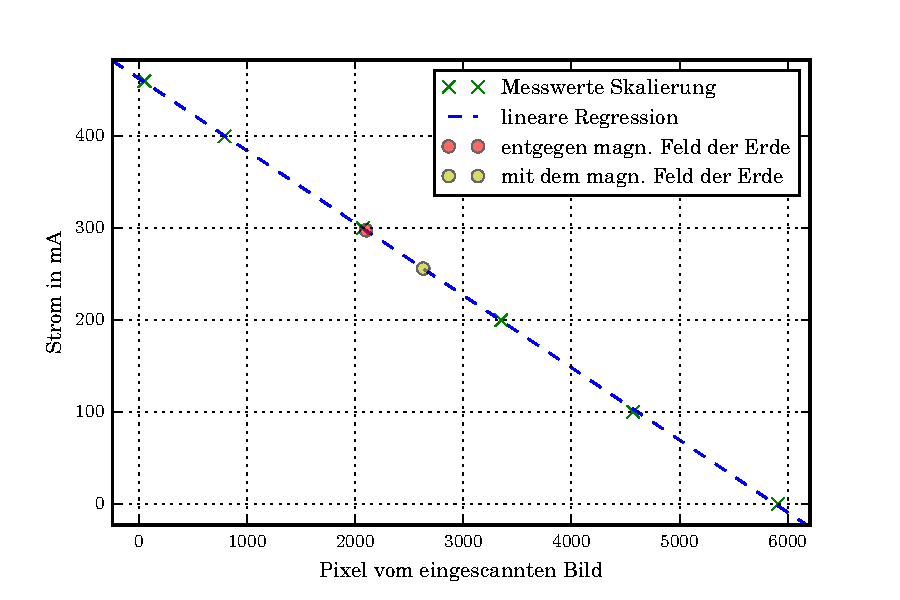
\includegraphics[width=\textwidth]{picture/10MHz.jpg}
     \caption{10 MHz}
     \label{fig:10Skiz}
  \end{subfigure}
  \begin{subfigure}[b]{0.49\textwidth}
     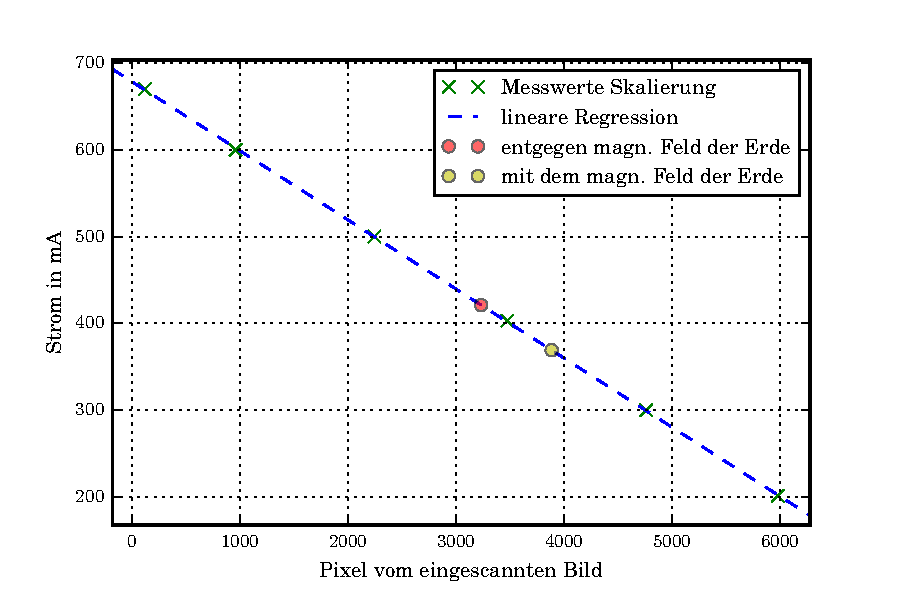
\includegraphics[width=\textwidth]{picture/15MHz.jpg}
     \caption{15 MHz}
     \label{fig:15Skiz}
  \end{subfigure}
  \begin{subfigure}[b]{0.49\textwidth}
     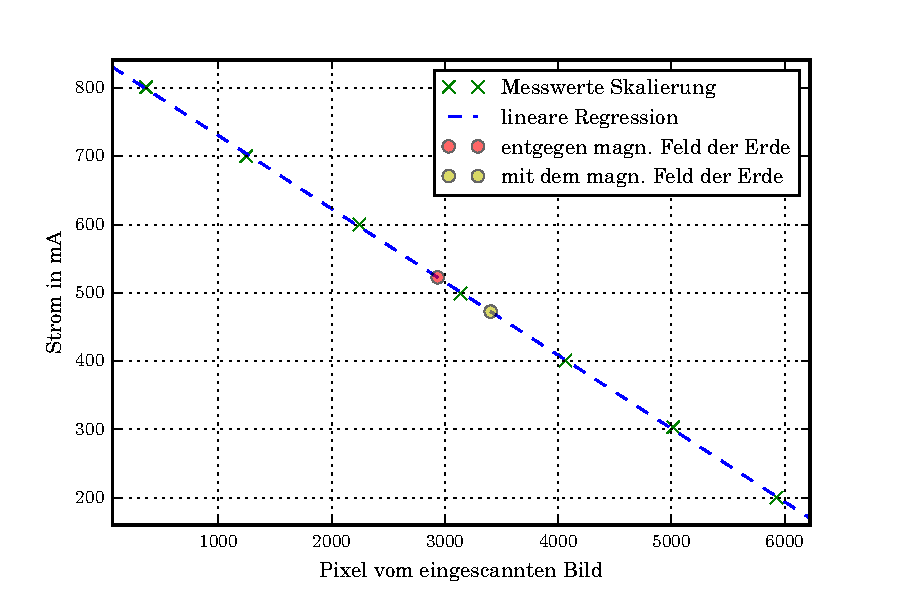
\includegraphics[width=\textwidth]{picture/20MHz.jpg}
     \caption{20 MHz}
     \label{fig:20Skiz}
  \end{subfigure}
  \begin{subfigure}[b]{0.49\textwidth}
     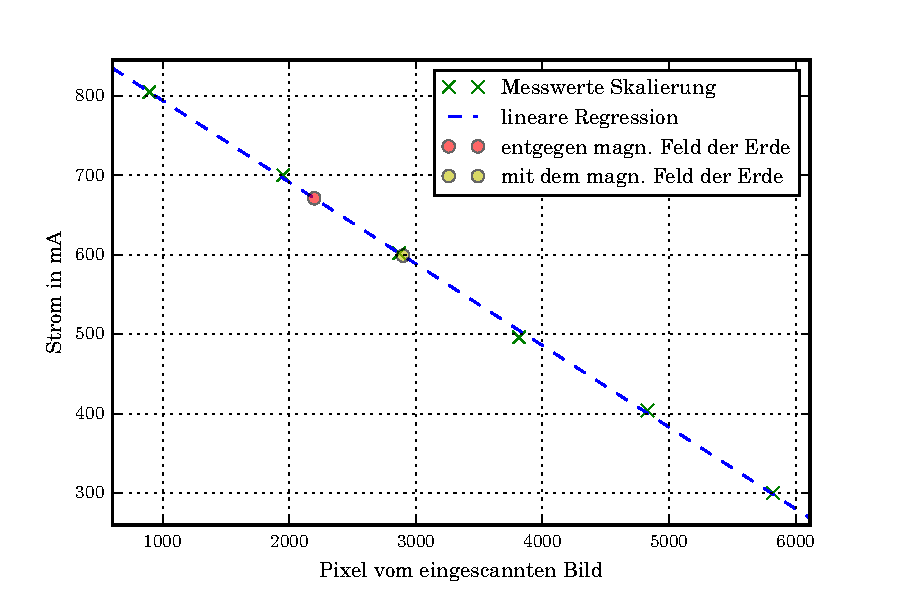
\includegraphics[width=\textwidth]{picture/25MHz.jpg}
     \caption{25 MHz}
     \label{fig:25Skiz}
  \end{subfigure}
  \begin{subfigure}[b]{0.49\textwidth}
     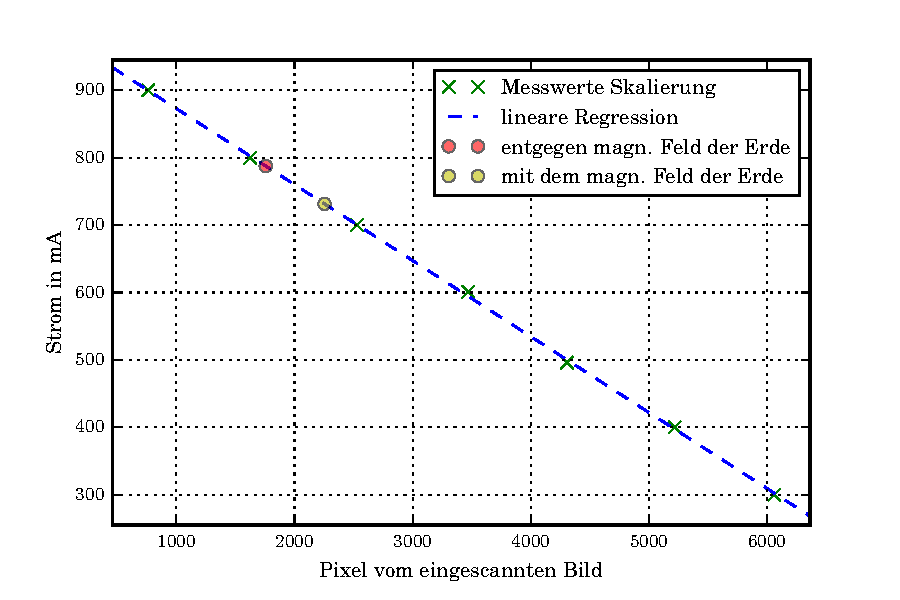
\includegraphics[width=\textwidth]{picture/30MHz.jpg}
     \caption{30 MHz}
     \label{fig:30Skiz}
  \end{subfigure}
  \caption{Brückenstrom in abhängigkeit des Spulenstrom für verschiedene $\nu_\text{Osz}$}
  \label{fig:Skizze}
\end{figure}
Dazu werden die Graphen eingescannt. Mittels den zuvor bestimmten kalibrierungspunkten wird die Pixelzahlen gegen den Spulenstrom aufgetragen und eine linearen Regression durch die Messpunkte gelegt.  
\begin{table}
  \centering
  \caption{Pixelzahl in abhängigkeit des Spulenstroms}
  \begin{tabular}{c c|c c|c c}
    \toprule
    	$I_{10 MHz}$ / mA & Pixel & $I_{15MHz}$ / mA & Pixel & $I_{20MHz}$ / mA & Pixel \\    
    \midrule
	0   & 5911 & 201 & 5980 & 200 & 5928 \\
	100 & 4572 & 300 & 4763 & 303 & 5018 \\
	200 & 3351 & 403 & 3477 & 401 & 4064 \\
	300 & 2070 & 500 & 2245 & 499 & 3138 \\
	400 & 792  & 600 & 960  & 600 & 2245 \\
	460 & 52   & 670 & 120  & 700 & 1246 \\
	--- & ---  & --- & ---  & 801 & 362  \\
    \bottomrule 
  \end{tabular}
  \label{tab:Mess}
\end{table}
\begin{table}
  \centering
  \caption{<+Caption text+>}
  \begin{tabular}{c c|c c}
    \toprule
 	$I_{25MHz}$ / mA & Pixel & $I_{30MHz}$ / mA & Pixel \\
    \midrule
	300 & 5823 & 300 & 6062 \\
	404 & 4830 & 400 & 5220 \\
	496 & 3815 & 496 & 4308 \\
	602 & 2870 & 601 & 3470 \\
	700 & 1953 & 700 & 2528 \\
	805 & 896  & 800 & 1624 \\
	--- & ---  & 900 & 762  \\
    \bottomrule
  \end{tabular}
  \label{tab:<+label+>}
\end{table}<++>
Anhand der Steigunung $m$ und des Bios $b$ der linearen Regression
\begin{equation}
  f(x) = m \cdot x + b
  \label{eqn:Reg}
\end{equation}
ergeben sich die in Tabelle \ref{tab:??} aufgeführten Koeffizienten. 
\begin{table}
  \centering
  \caption{}
  \begin{tabular}{c|c c}
    \toprule
    	$\nu_\text{Osz}$ & Steigung m & Bios b \\
    \midrule
       	10 MHz & \num{7.87 +- 0.04}  & \num{463 +- 1.4} \\
	15 MHz & \num{7.97 +- 0.03}  & \num{678.6 +- 1.1} \\ 
	20 MHz & \num{10.73 +- 0.07} & \num{837 +- 2} \\
	25 MHz & \num{10.2 +- 0.1}   & \num{897 +- 5} \\
	30 MHz & \num{11.27 +- 0.08} & \num{986 +- 3.3}\\
    \bottomrule
  \end{tabular}
  \label{tab:}
\end{table}

\begin{table}
  \centering
  \caption{}
  \begin{tabular}{c|c c c}
    \toprule
    \multirow{2}{*}{$\nu_\text{Osz}$} & B-Feld in Richtung & B-Feld entgen der Richtung & gemitteltes \\
    	& des Erdmagnetfeld / $\mu T$ & des Erdmagnetfeld / $\mu T$ & B-Feld / $\mu T$ \\
    \midrule
       	10 MHz & \num{417 +- 2} & \num{359 +- 3} & \num{388 +- 2} \\
	15 MHz & \num{590 +- 2} & \num{518 +- 2} & \num{554 +- 2} \\ 
	20 MHz & \num{733 +- 4} & \num{663 +- 5} & \num{698 +- 4} \\
	25 MHz & \num{941 +- 8} & \num{840 +- 8} & \num{891 +- 8} \\
	30 MHz & \num{1105 +- 5} & \num{1026 +- 5} & \num{1066 +- 5} \\
    \bottomrule
  \end{tabular}
  \label{tab:}
\end{table}

\begin{table}
  \centering
  \caption{}
  \begin{tabular}{c|c c}
    \toprule
    	$\nu_\text{Osz}$ & Erdmagnetfeld / \mu T & Lande Faktor \\
    \midrule
       	10 MHz & \num{29.2 +- 0.2} & \num{1.95 +- 0.01} \\
	15 MHz & \num{36.5 +- 0.1} & \num{2.06 +- 0.01} \\ 
	20 MHz & \num{35.1 +- 0.2} & \num{2.10 +- 0.01} \\
	25 MHz & \num{50.6 +- 0.6} & \num{2.01 +- 0.02} \\
	30 MHz & \num{39.4 +- 0.3} & \num{2.01 +- 0.01} \\
    \bottomrule
  \end{tabular}
  \label{tab:}
\end{table}

\begin{figure}
  \centering
  \begin{subfigure}[b]{0.49\textwidth}
     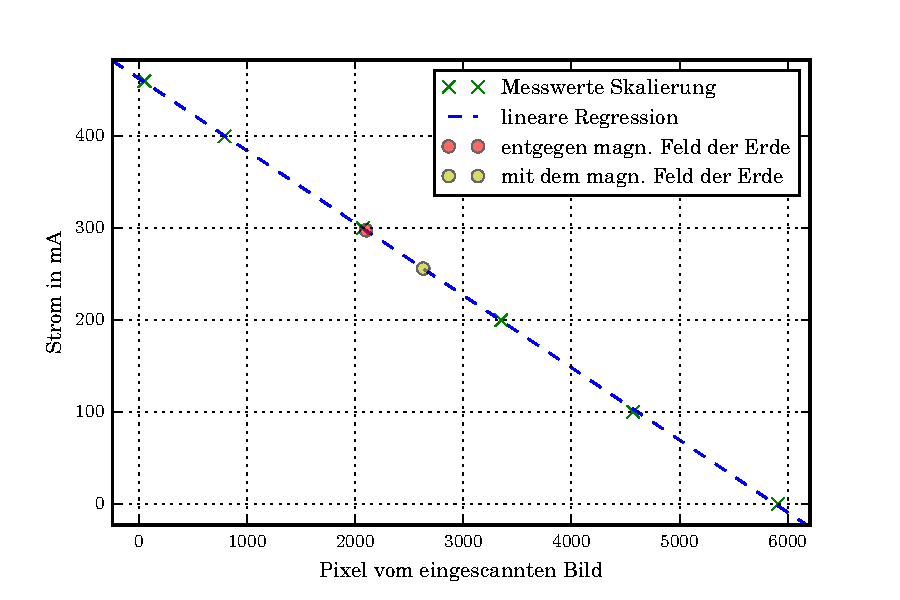
\includegraphics[width=\textwidth]{picture/10MHz.pdf}
     \caption{10 MHz}
     \label{fig:10Reg}
  \end{subfigure}
  \begin{subfigure}[b]{0.49\textwidth}
     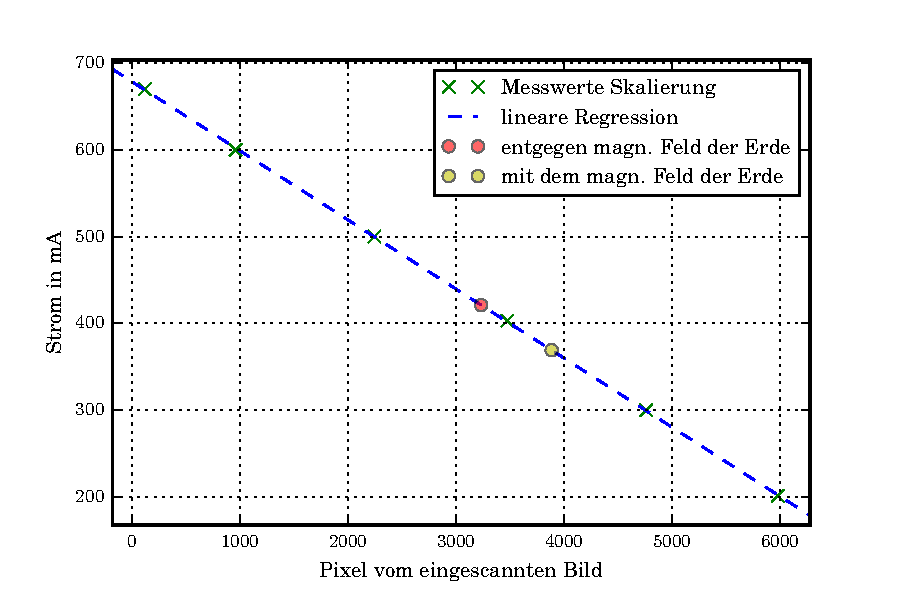
\includegraphics[width=\textwidth]{picture/15MHz.pdf}
     \caption{15 MHz}
     \label{fig:15Reg}
  \end{subfigure}
  \begin{subfigure}[b]{0.49\textwidth}
     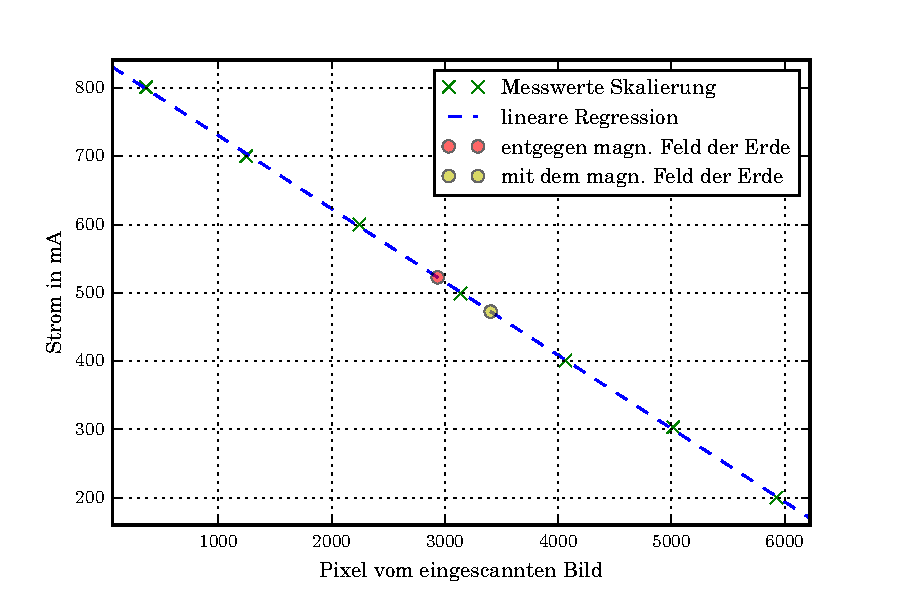
\includegraphics[width=\textwidth]{picture/20MHz.pdf}
     \caption{20 MHz}
     \label{fig:20Reg}
  \end{subfigure}
  \begin{subfigure}[b]{0.49\textwidth}
     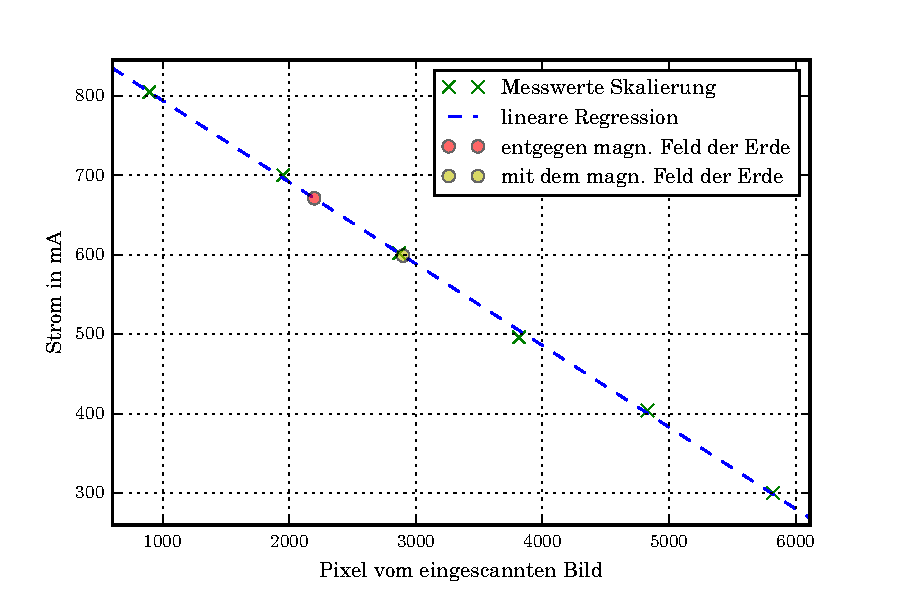
\includegraphics[width=\textwidth]{picture/25MHz.pdf}
     \caption{25 MHz}
     \label{fig:20Reg}
  \end{subfigure}
  \begin{subfigure}[b]{0.49\textwidth}
     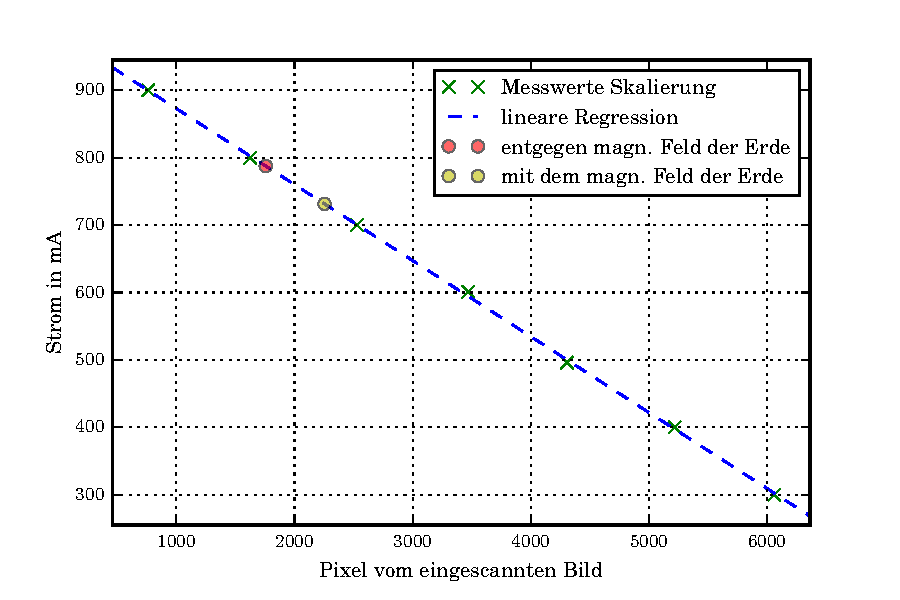
\includegraphics[width=\textwidth]{picture/30MHz.pdf}
     \caption{30 MHz}
     \label{fig:30Reg}
  \end{subfigure}
  \caption{Lineare Regression zwischen der Pixel und des Spuelnstroms für unterschiedliche Frequenzen}
  \label{fig:Reg}
\end{figure}
